\chapter{Introducción Específica} % Main chapter title

\label{Chapter2}

Es este capítulo se presentarán las topologías básicas del sistema ferroviario y los dos enfoques de resolución del proyecto, con sus ventajas y desventajas antes de abordar la implementación de la solución elegida.

\section{Topologías típicas}
	
	El tendido ferroviario argentino dista de ser uniforme: en las zonas rurales predominan vías simples con bypass debido al alto costo de utilizar vías dobles, mientras que en las zonas urbanas son mayoría las estaciones y playas de maniobras a talleres de mantenimiento.
	
	Es por eso que el trabajo realizado debe abocarse a muchos frentes y muy diversos unos de otros. La cantidad de elementos involucrados diverge conforme la complejidad de la topología se incrementa, pero los elementos y sus comportamientos no dejan de ser los mismos de los presentados en el Capítulo 1.

	\subsection{Bypass}

		Para cubrir grandes distancias entre un punto estratégico como podría ser Vaca Muerta y un puerto para la exportación de los recursos es necesaria una línea ferroviaria con vagones de carga que puedan transportar el producto. Es obvio que es necesario un ida y vuelta entre trenes vacíos que van a ser llenados en el destino y trenes llenos que van a descargar al puerto la carga que lleven, pero el costo de utilizar dos vías en sentidos opuestos es muy elevado y utilizar solo un no tiene el menor sentido logístico.
		
		Es por eso que se utiliza la topología de bypass cada cierta cantidad de kilómetros de vía simples para poder permitir que trenes en sentidos opuestos se crucen sin riesgo de colisión. Se presenta en la Figura \ref{fig:Bypass} una representación de la topología bypass donde un tren que circula hacia la derecha por la vía principal podría entrar en colisión lateral con un tren que busca ingresar a la red desde una vía secundaria por medio del cambio de vías.
		
		\begin{figure}[h]
		\centering
			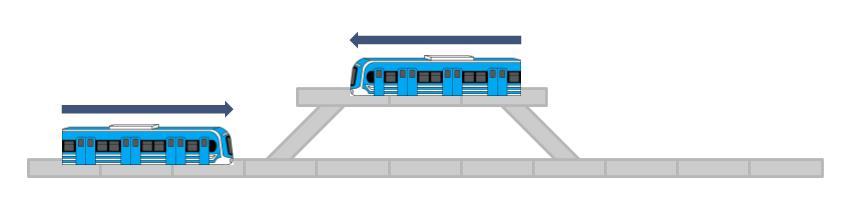
\includegraphics[scale=.5]{./Figures/Bypass_2}
			\caption{Topología bypass}
			\label{fig:Bypass}
		\end{figure}
			
	\subsection{Estación}

		Explicacion
		
			\begin{figure}[h]
			\centering
				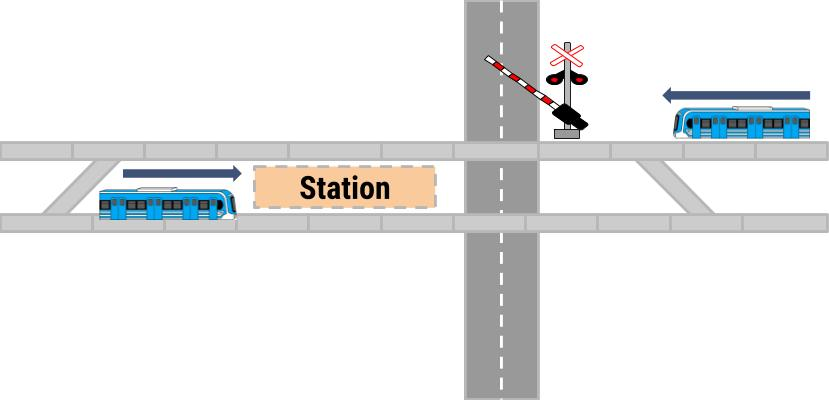
\includegraphics[scale=.5]{./Figures/Estacion}
				\caption{Topología estación}
				\label{fig:Estacion}
			\end{figure}

	\subsection{Hub}
	
		Explicacion
		
			\begin{figure}[h]
			\centering
				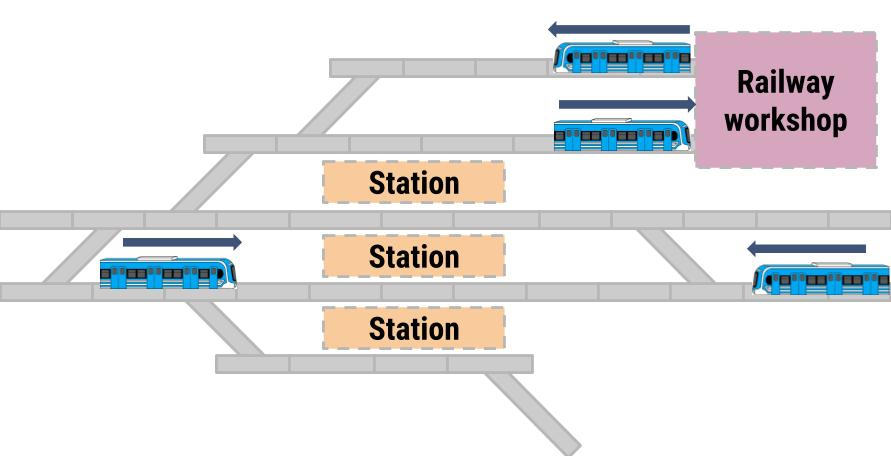
\includegraphics[scale=.45]{./Figures/Hub}
				\caption{Topología hub}
				\label{fig:Hub}
			\end{figure}
	
	\subsection{Terminal}
		
		Explicacion
		
			\begin{figure}[h]
			\centering
				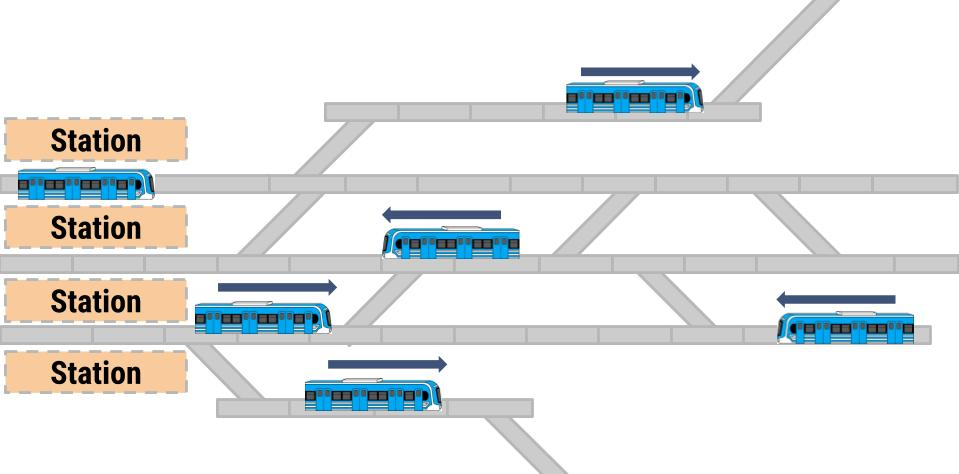
\includegraphics[scale=.4]{./Figures/Terminal}
				\caption{Topología terminal}
				\label{fig:Terminal}
			\end{figure}
		
		Explicacion
							
\section{Enfoque funcional}

	Explicacion
	
		\begin{figure}[h]
		\centering
			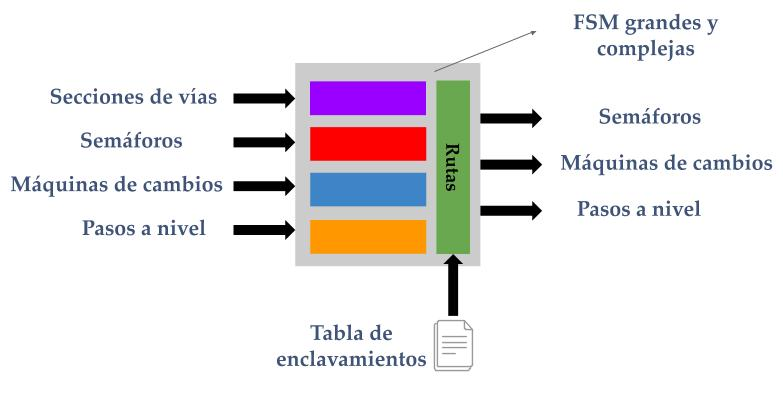
\includegraphics[scale=.55]{./Figures/Funcional}
			\caption{Enfoque funcional}
			\label{fig:Funcional}
		\end{figure}
	
	Explicacion
			
		\begin{figure}[h]
		\centering
			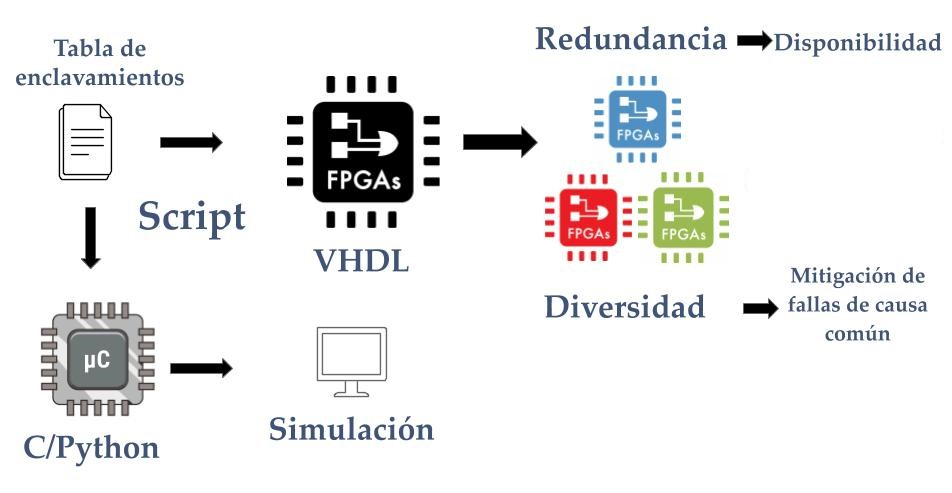
\includegraphics[scale=.4]{./Figures/Funcional_workflow}
			\caption{Esquema de trabajo en el enfoque funcional}
			\label{fig:Funcional}
		\end{figure}
	
	Explicacion
			
		\begin{figure}[h]
		\centering
			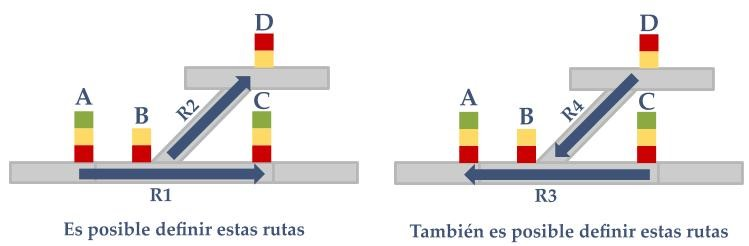
\includegraphics[scale=.4]{./Figures/Tablas}
			\caption{Ejemplo de elaboración de tabla de enclavamientos}
			\label{fig:EJ_Tabla}
		\end{figure}
	
	Explicacion		
			
		\begin{figure}[h]
		\centering
			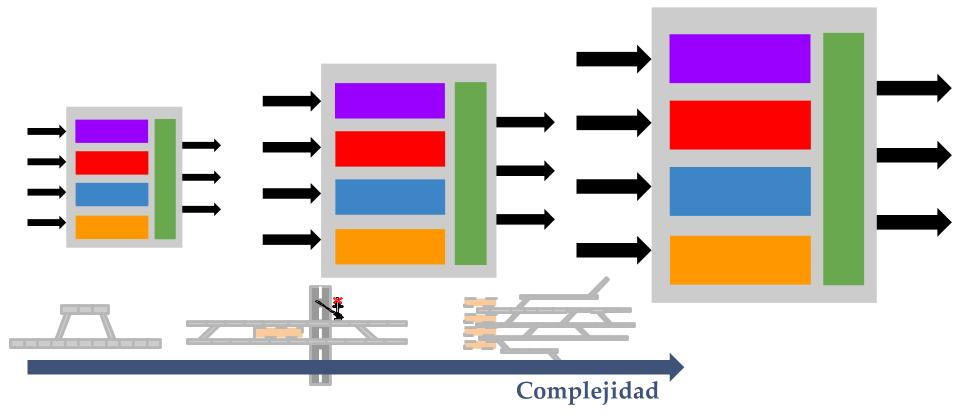
\includegraphics[scale=.4]{./Figures/Funcional_complejidad}
			\caption{Escalabilidad del enfoque funcional}
			\label{fig:Funcional}
		\end{figure}
		
	Explicacion
			
\section{Enfoque geográfico}

	Explicacion
	
		\begin{figure}[h]
		\centering
			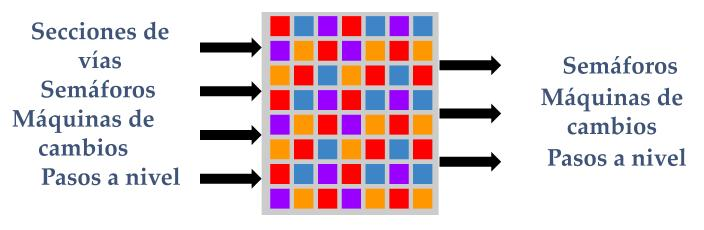
\includegraphics[scale=.55]{./Figures/Geografico}
			\caption{Enfoque geográfico}
			\label{fig:Geografico}
		\end{figure}

	Explicacion
		
		\begin{figure}[h]
		\centering
			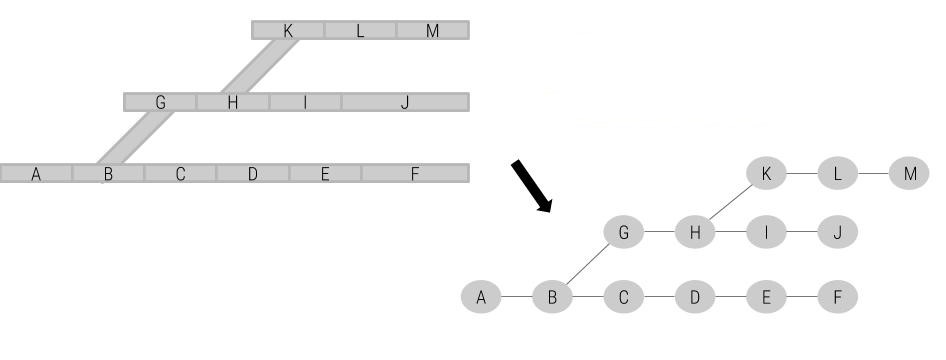
\includegraphics[scale=.4]{./Figures/Topologia_grafo}
			\caption{Pasaje de topología ferroviaria a grafo}
			\label{fig:Funcional}
		\end{figure}
	
	Explicacion
	
		\begin{figure}[h]
		\centering
			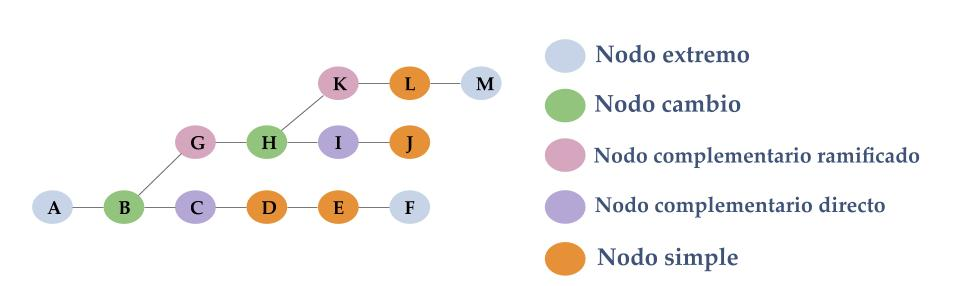
\includegraphics[scale=.4]{./Figures/Grafo}
			\caption{Análisis del grafo ferroviario}
			\label{fig:Funcional}
		\end{figure}
	
	Explicacion
		
		\begin{figure}[h]
		\centering
			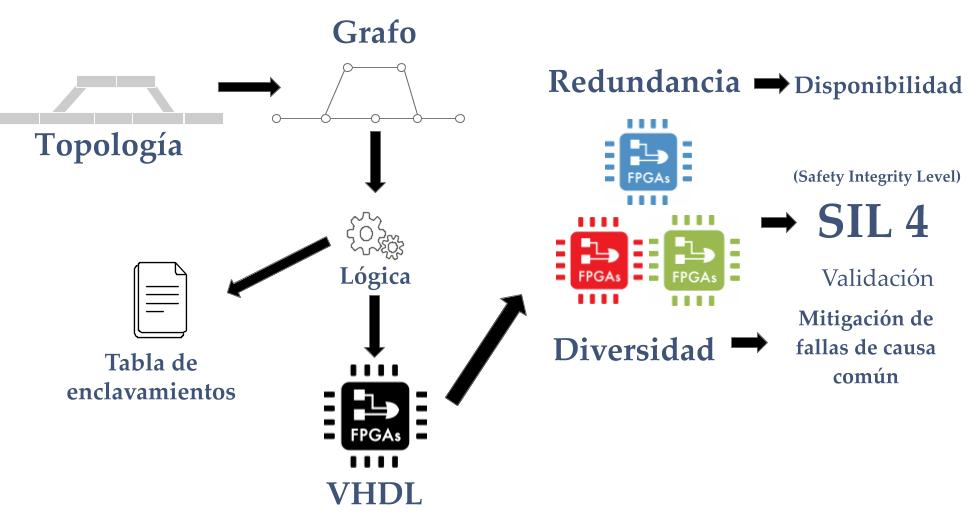
\includegraphics[scale=.4]{./Figures/Geografico_workflow}
			\caption{Esquema de trabajo en el enfoque geográfico}
			\label{fig:Funcional}
		\end{figure}
	
	Explicacion
			
		\begin{figure}[h]
		\centering
			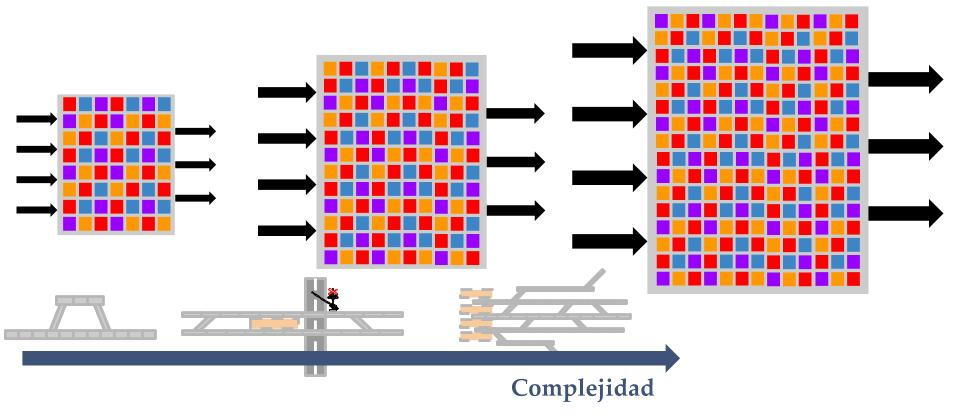
\includegraphics[scale=.4]{./Figures/Geografico_complejidad}
			\caption{Escalabilidad del enfoque geográfico}
			\label{fig:Funcional}
		\end{figure}
		
	Explicacion